\section{Introduction}
% Citation needed for self-consistency and its sampling-and-voting procedure.
Self-consistency samples several reasoning trajectories and aggregates their answers.
Its cost grows with the amount of generated reasoning. Even when early samples have found a useful intermediate calculation, later trajectories ordinarily start again from the original question. This suggests reusing part of an earlier solution while continuing to sample diverse suffixes. The potential saving comes from generating less new text per trajectory. Figure~\ref{fig:overview} illustrates the observed repetition and contrasts independent sampling with shared-prefix reuse.

\begin{figure}[t]
\centering
% Author-supplied PDFs are included unchanged and retain vector graphics.
% Bottom alignment places the (b) and (c) caption baselines at the same height.
\begin{minipage}[b]{0.435\linewidth}
\centering
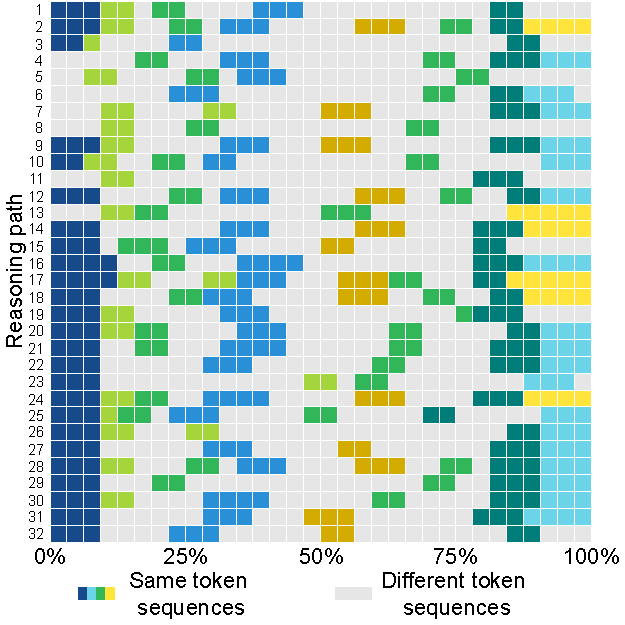
\includegraphics[width=\linewidth]{figs/SC_matrix.pdf}
\par\smallskip
{\small\textbf{(a) SC: independently sampled paths}}
\par\medskip
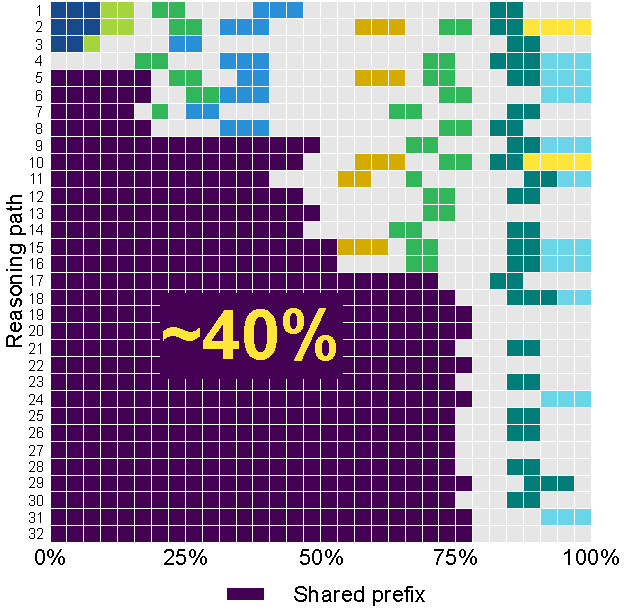
\includegraphics[width=\linewidth]{figs/PC_matrix.pdf}
\par\smallskip
{\small\textbf{(b) PC: shared-prefix reuse}}
\end{minipage}\hfill
\begin{minipage}[b]{0.545\linewidth}
\centering
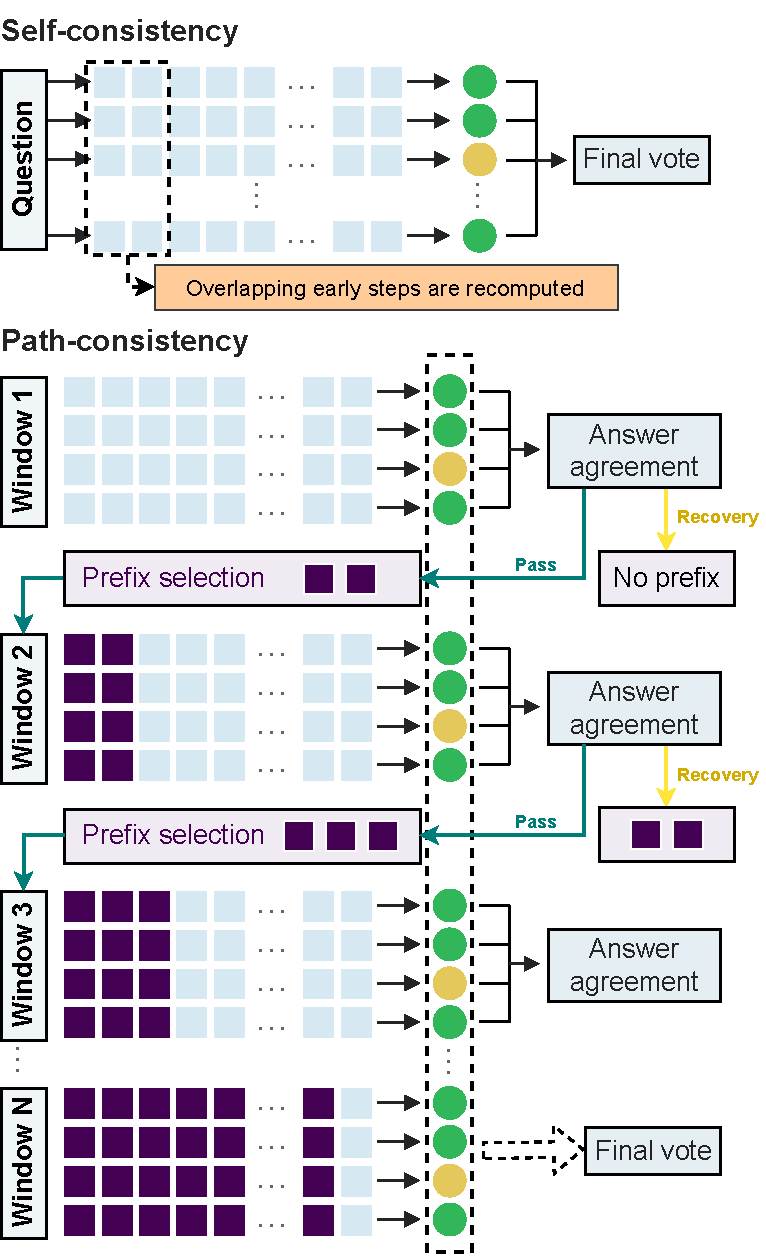
\includegraphics[width=\linewidth]{figs/overview.pdf}
\par\smallskip
{\small\textbf{(c) Overview of SC and PC}}
\end{minipage}

% Citations may be added for GSM8K and Llama-3.1 at their first formal introduction.
% The repetition visualization and token-saving result are evidence from our experiments.
\caption{From repeated reasoning to shared-prefix reuse. (a,b) SC and PC on the same GSM8K question using Llama-3.1-8B-Instruct. Each matrix shows 32 reasoning paths over 32 relative token intervals. Matching colors mark repeated token sequences, purple marks shared prefixes, and gray marks other content. The $\sim$40\% denotes average token savings on GSM8K. (c) SC samples independent paths, whereas PC progressively reuses prefixes across windows. Circles represent answers, with colors indicating answer categories.}
\label{fig:overview}
\end{figure}

We propose path-consistency, a method for token-efficient reasoning through controlled prefix reuse across sampling windows. After a window finishes, answer agreement determines whether to propose a prefix extension. Path-consistency selects a continuous prefix from a trajectory supporting the modal answer and uses it to condition the next window. Subsequent windows test whether to commit the proposal or recover an earlier prefix. Later trajectories therefore reuse part of the reasoning already generated and sample new continuations, while all valid answers contribute to the final vote.

Path-consistency has three practical advantages. First, it reduces the amount of new reasoning generated per trajectory while retaining multiple sampled continuations and answer aggregation. Second, it requires no training, fine-tuning, or architectural changes, operating entirely at inference time through answer agreement, prefix selection, and trial and recovery. Third, prefix reuse is compatible with different autoregressive language models and can be combined with early-stopping methods for additional token savings. These properties make path-consistency a flexible component for efficient multi-path reasoning.

% Citations may be added for the evaluated models and benchmarks at their formal introduction.
% Citations needed for reasoning-sharing and early-stopping baselines at their formal introduction.
% The evaluation overview uses the intended complete-paper framing. Verify Qwen coverage against the final tables before submission.
% The numerical range and mean below refer only to Llama/GSM8K and the four DeepSeek main-table comparisons, not to pending Qwen results.
We evaluate path-consistency using three models of different scales, Llama-3.1-8B-Instruct, DeepSeek-V4-Flash, and Qwen3-30B-A3B, across five reasoning benchmarks. We first examine how shared prefixes progressively extend across sampling windows on Llama-3.1 and GSM8K, then present the main results on DeepSeek and Qwen. On Llama/GSM8K and the four DeepSeek main-table benchmarks, path-consistency reduces generated tokens by 25.8\% to 39.4\%, averaging 30.8\% across these settings, while largely maintaining accuracy. Comparisons with reasoning-sharing methods assess path-consistency's accuracy and token efficiency, and combinations with early-stopping methods demonstrate additional savings. Finally, ablation studies examine the roles of source selection and recovery, as well as how the answer agreement threshold governs prefix reuse and informs operating-point selection.
